\section{Preliminaries}
For $m,n,r\in\bbN$ we write $m =_r n$ iff $m=n$ or $m,n>r$.

\subsection{Graphs}
Let $\frakG=(V,E)$ be a graph (possibly with some constants $c_1,\dots,c_n\in V$). 
For $u,v\in V$ we denote by $d^\frakG(u,v)$ the length of a shortest path from $u$ to $v$, where we set $d(u,v) = \infty$ whenever $u$ and $v$ are not connected in $\frakG$.
For $A\subseteq V$ we denote by $\frakG_{\upharpoonright A}$ the induced subgraph of $\frakG$ with vertex set $A$. 
For a nonempty set $A\subseteq V$ and $r\in \bbN$ let $\calN_r^\frakG(A)$ denote the \emph{$r$-neighborhood} of $A$ (and the constants $c_1,\dots,c_n$) in $\frakG$, that is $\frakG_{\upharpoonright\{u\in V\mid \min\{d(u,v) \mid v\in A\cup\{c_1,\dots,c_n\}\} \leq r \}}$.
For a tuple $\vec{u} = (u_1,\ldots, u_k) \in V^k$ we will also write $\calN^\frakG_r(\vec{u})$ instead of $\calN^\frakG_r(\{u_1,\ldots, u_k\})$.

\subsection{Combinatorics on Words}
Let $\Sigma$ be an alphabet. We use $\preceq$ to denote the \emph{prefix-relation} and $\sqsubseteq$ for the \emph{suffix-relation} on $\Sigma^\ast$.  If $u= vw$ we write $v^{-1}u = w$ and
$uw^{-1} = v$.
Let $\pref_r(u)$ denote the maximal prefix of $u$ of length at most $r$. For $u,v\in\Sigma^\ast$ let $u \sqcap v$ denote the largest suffix of $u$ that is also a prefix of $v$.

In a first lemma we prove that the complementary prefix and suffix of $u$ resp.~$v$ wrt.~$u\sqcap v$ can be shortened to words of length at most $2r$ having the same prefixes and suffixes:

\begin{lemma}\label{lem:short_ends_construction}
	Let $r\in\bbN$ and $u,v,w \in\Sigma^\ast$ with $uw\sqcap wv = w$. %such that the period of $w$ has length at least $2$. 
	Then there are words $u',v'$ of length $\calO(r)$ such that 
	\begin{itemize}
		\item $\suf_r(uw) = \suf_r(u'w)$,
		\item $\suf_r(wv) = \suf_r(wv')$,
		\item $\pref_r(wv) = \pref_r(wv')$,
		\item $u'w\sqcap wv' = w$.
	\end{itemize}
\end{lemma}
\begin{proof}
	Set $u'=\suf_r(u)$. Additionally, if $|v|\leq 2r$ set $v':=v$, and otherwise, set $v':=\pref_r(v)\suf_r(v)$. Then the first three equations are obviously satisfied. Now assume $u'w\sqcap wv'\neq w$, i.e., there is $w'\in \Sigma^*$ with $|w'|>|w|$, $w'\preceq wv'$, and $w'\sqsubseteq u'w$. Since $|u'w|\leq r+|w|$ we have $w'\preceq w\pref_r(v)\preceq wv$. Additionally, we have $w'\sqsubseteq u'w\sqsubseteq uw$ implying $|uw\sqcap wv|\geq|w'|>|w|$. This is a contradiction to the definition of~$w$.
\end{proof}

A \emph{period} of a word $u$ is a word $v$ such that $u \preceq v^\omega$. Obviously every word $u$ has a unique smallest period, which we denote by $\root{u}$. The \emph{left-exponent} of $u$ in $v$ is the largest number $n$ such that $v= u^nw$, and it is denoted by $\lexp(u,v)$. The \emph{right-remainder}, $v\mod u$,  of $v$ with respect to $u$ is defined as $(u^{\lexp(u,v)})^{-1}v$, that is the unique $w$ such that $v= u^{\lexp(u,v)}w$.  In particular we have $v= \root{v}^{\lexp(\root{v}, v)}(v \mod \root{v})$ for every $v\in\Sigma^\ast$. A word $u$ is \emph{primitive} if there is no $v$ with
$|v| < |u|$ and $u = v^n$ for some $n\in\bbN$.
For $u,v\in\Sigma^\ast$ let $u\Delta v = (y,z)$, where $y,z$ are minimal such that there exists an $x$ with $u=xy$ and $v=xz$. For $\vec{v}, \vec{w}\in(\Sigma^\ast)^k$ let 
$\vec{v}\Delta\vec{w} = (v_1\Delta w_1,\ldots, v_k\Delta w_k) \in (\Sigma^\ast)^{2k}$ and $|\vec{w}| \coloneq \sum_{i=1}^{k}|w_i|$. 

\begin{definition}
	Let $u\in \Sigma^\ast$ be a word. A \emph{canon-decomposition} of $u$ is a sequence of words $\epsilon = u_0,u_1,\ldots, u_n = u$ such that for all $0\leq i < n$ it holds that
	$u_i \precneq u_{i+1}$ and $u_i \sqsubsetneq u_{i+1}$ ($u_i \presuf u_{i+1}$ for short). A canon-decomposition $u_0,u_1,\ldots, u_n $ is \emph{complete} if there is no $1\leq i< n$ and $v\in\Sigma^\ast$ with $u_i \presuf v \presuf u_{i+1}$.
\end{definition}

\begin{lemma}
	Every word $w\in\Sigma^\ast$ has a unique complete canon-decomposition.
\end{lemma}
\begin{proof}
	Obviously, every word $w$ possesses at least one complete canon-decomposition. Now suppose $\vec{u} = (u_0,\ldots,u_m)$ and $\vec{v}=(v_0,\ldots,v_n)$ are two distinct complete canon-decompositions of
	a word $w\in\Sigma^\ast$. W.l.o.g. assume that $n \leq m$. We claim that there is an $0\leq i \leq n$ with $u_i \neq v_i$. Because otherwise it follows from $w= u_n = v_n$ that    
	$\vec{u}$ and $\vec{v}$ have the same length $n$ and this, in turn, implies that they are identical since $u_i=v_i$ for all $0\leq i\leq n$. Now choose the smallest $i$ between $0$ and $n$ such that $u_i \neq v_i$. As $u_0 = \epsilon = v_0$ it holds that $i>0$. Hence $u_{i-1}, v_{i-1}$ are defined and $u_{i-1} = v_{i-1}$. Since $u_i, v_i \preceq w$ and $u_i \neq v_i$ it must be the case that $|u_i| \neq |v_i|$. Again w.l.o.g. assume that $|u_i| < |v_i|$. Then  $u_i, v_i \preceq w$, $u_i, v_i \sqsubseteq w$ and $|u_i| < |v_i|$, which implies $u_i \presuf v_i$. Therefore 
	$v_{i-1} = u_{i-1} \presuf u_i \presuf v_i$ in contradiction to the completeness of $\vec{v}$!
\end{proof}

\begin{example}
	The  complete canon-decomposition of $ababa$ is $(\epsilon, a, aba, ababa)$.
\end{example}

%\begin{definition}
%	A word $u$ is \emph{periodic} if $u=v^n$ for some $v\in\Sigma^+$ and $n>1$. Otherwise $u$ is primitiv. We say that $u$ is almost periodic if $u= (vw)^nv$ for some $n\geq 1$,  $v\in \Sigma^\ast$, and $w\in\Sigma^+$.  We write $\sqrt{u}^{\ast}$ for the unique pair $(v,w) \in \Sigma^\ast\times\Sigma^+$ such that
%   $vw$ is primitive and $u = (vw)^nv$ for some $n\geq 1$.
%
%\end{definition}

%\begin{lemma}
%	Let $\vec{u} = (u_0,\ldots,u_n)$ be a complete canon-decomposition. Then $\root{u_{i+1}} = u_{i+1}u_i^{-1}$ for all $0\leq i < n$. 
%\end{lemma}
%\begin{proof}
%	Fix some $0\leq i < n$ and let $v:= u_{i+1}u_i^{-1}$. Let us verify first that $v$ is indeed a period of $u_{i+1}$. If $2|u_i| \leq |u_{i+1}|$ then $u_{i+1} = u_iwu_i$ for some $w\in\Sigma^\ast$. 
%	Hence $v= u_iw$ and $u_{i+1} \preceq (u_iw)^\omega = v^\omega$. Otherwise  $2|u_i| > |u_{i+1}|$ and therefore the $u_i$-prefix and the $u_i$-suffix of $u_{i+1}$ overlap. We can use this overlap to 
%	show via a simple induction that the situation is as depicted in Fig.~\ref{fig:root}.
%	\begin{figure}[h]
%		\centering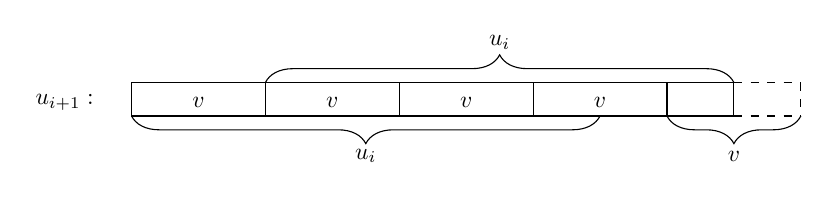
\begin{tikzpicture}[scale=0.85,every node/.style={scale=0.85}]
	\node at (-1, .2) {$u_{i+1}:$};
	\node at (1, .2) {$v$};
	\node at (3, .2) {$v$};
	\node at (5, .2) {$v$};
	\node at (7, .2) {$v$};
	\draw [decorate,decoration={brace,amplitude=10pt}] (10,0) -- (8, 0) node [black,midway,yshift=-.6cm] {$v$};
	\draw (0,0) rectangle (9, .5);
	\draw [decorate,decoration={brace,amplitude=10pt}] (7,0) -- (0, 0) node [black,midway,yshift=-.6cm] {$u_i$};
	\draw [decorate,decoration={brace,amplitude=10pt}] (2,0.5) -- (9, 0.5) node [black,midway,yshift=.6cm] {$u_i$};
	\draw (2,.5) -- (2,0);
	\draw (4,.5) -- (4,0);
	\draw (6,.5) -- (6,0);
	\draw (8,.5) -- (8,0);
	\draw[dashed] (10,.5) -- (10,0);
	\draw[dashed] (9,.5) -- (10,.5);
	\draw[dashed] (9,0) -- (10,0);   
\end{tikzpicture}
%		\caption{\label{fig:root}}
%	\end{figure}
%
%	Now suppose that $|\root{u_{i+1}}| < |v|$. Then let $u_i' \coloneq \root{u_{i+1}}^{\lexp(\root{u_{i+1}}, u_{i+1}) -1}(u_{i+1} \mod \root{u_{i+1}})$.
%	Then $u_i' \presuf u_{i+1}$ and $|u_i'| = |u_{i+1}| - \root{u_{i+1}} > |u_{i+1}| - |v| = |u_i|$. Hence $u_i\presuf u_i' \presuf u_{i+1}$ contradicting the completeness of $\vec{u}$! 
%\end{proof}

From the complete canon-decomposition of a word~$w$ we derive the so called skeleton of~$w$ containing the inner words $v$ of all canons $uvu$ in $w$.

\begin{definition}
	Let $w\in\varSigma^\ast$ and $\vec{w} = (w_0,\ldots,w_n)$ be the complete canon-decomposition of $w$. The \emph{$r$-skeleton} of $w$, denoted by $\calS_r(w)$, is the word of length $n$ over the alphabet $\Gamma = \Sigma^{\leq r}$ with $\calS_r(w)[i] = \pref_r(w_i^{-1}w)$ for each $0\leq i\leq n-1$. Note that $w_i^{-1}w$ is always defined since $w_i\preceq w$.
\end{definition}

\begin{example}
	Let $u= bababa$ and $v=ababab$. Then $u\sqcap v = ababa$ and the complete canon-decomposition of $u\sqcap v$ is $(\epsilon, a, aba, ababa)$. The $2$-skeleton of $u\sqcap v$ is the word depicted below.
	\begin{center}
		\begin{tikzpicture}[scale=0.85]
			\node[] (0) {$ab$};
			\node[ right=of 0] (1) {$ba$};
			\node[ right=of 1] (2) {$ba$};
			
			\path[ ->,>=latex'] (0) edge (1)
			(1) edge (2);
		\end{tikzpicture}
	\end{center}
\end{example}

By definition the $i$-th element of the canon decomposition of  $u\sqcap v$ corresponds to the $i$-th letter of the skeleton. We will use this correspondence to translate back and forth between 
an Ehrenfeucht-Fra\"{\i}ss\'{e} game played on the Cayley-graph of a queue monoid and games played on certain skeletons which are derived from the game played on the Cayley-graph. 

\begin{lemma}\label{lem:short_from_skeleton}
	Let $r\in\bbN$, $w\in\Sigma^*$ and $n\in\bbN$ be the length of $\calS_r(w)$. Then a word $v\in\varSigma^*$ can be constructed from $w$ such that $|v|=\calO(2^{nr})$ and $\calS_r(w)=\calS_r(v)$.
\end{lemma}
\begin{proof}
	Let $\vec{w}=(w_0,\dots,w_n)$ be the complete canon-decomposition of~$w$. At first, assume $|\calS_r(w)[n-1]|<r$ (i.e., the last component is small). Then there are two possibilities: on the one hand $w=w_{n-1}xw_{n-1}$ and $|xw_{n-1}|<r$. In this case we have $|w|<2r=\calO(2^{nr})$. On the other hand we have $w=xw_{n-1}=w_{n-1}y$ where $|x|=|y|<\min\{|w_{n-1}|,r\}$, i.e., the prefix and the suffix $w_{n-1}$ overlap in $w_n$. Then it is easy to see that $x$ is a period of $w_{n-1}$ and of $w_n$. Concretely, there is a prefix $p$ of $x$ and a number $k\in\bbN$ such that $w=x^kp$ and $w_{n-1}=x^{k-1}p$. In particular, all word $x^ip$ with $1\leq i\leq k$ are borders of $w$ which implies $k\leq n$. Hence we have $|w|\leq|x|\cdot(k+1)\leq r\cdot(n+1)=\calO(2^{nr})$. Therefore, in both cases we are ready and we can assume $|\calS_r(w)[n-1]|$ from now on.
	
	We construct~$v$ inductively as follows: We set $v_0:=\epsilon$. Now let $a,b\in\varSigma$ be distinct with $\calS_r(w)[0]\in a\varSigma^*$. Then $x\presuf\calS_r(w)[0]b^{2n+r}$ implies $x=\epsilon$. Hence, we set, for $0\leq i<n$, $v_{i+1}:=v_ix_iv_i$ where $x_i=\calS_r(w)[i]\,b^{n-i}a^ib^{n+r}$. Finally, we set $v:=v_{n}$.
	
	Before we can prove $\calS_r(w)=\calS_r(v)$ we need to prove the following two properties of $(v_0,\dots,v_n)$:
	\begin{alphaenumerate}
		\item For each $0\leq i\leq n$ $\root{v_{i+1}}=v_ix_i$ and\label{prf:short_from_skeleton:i1}
		\item $\vec{v}=(v_0,\dots,v_{n})$ is a complete canon-decomposition of $v$.\label{prf:short_from_skeleton:i2}
	\end{alphaenumerate}
	
	\emph{Proof of (\ref{prf:short_from_skeleton:i1}).}\ We observe that $v_ix_i$ is a period of $v_{i+1}$ and we prove by induction on $0\leq i\leq n$ that this period is minimal. For $i=0$ this is trivial since $v_1\in a\varSigma^{r-1}b^{2n+r}$ and $a\neq b$. So now let $i>0$. We suppose that there is a period $p$ of $v_{i+1}$ with $|p|<|v_ix_i|$. Then, for $y_j:=x_j(b^{n+r})^{-1}$ for $0\leq j\leq i$, the word $v_{i+1}$ is an alternation of words $y_j$ and $b^{r+n}$ which are all of length $r+n$. Note that by construction we have $y_{j}\neq b^{n+r}$ (since each $y_{j}$ contains at least one $a$) as well as $y_{j}\neq y_{k}$ if $j\neq k$ for each $0\leq j,k\leq i$. Additionally, each second occurrence of a $y_j$-block is $y_1$. We now consider two cases:
	
	First, assume that $|p|$ is not a divisor of $n+r$. If $|p|<n+r$ then the distance between each two occurrences of $a$ in $p^\omega$ is at most $|p|<n+r$ but $v_{i+1}$ contains at least one $b^{n+r}$-block. Hence, we have $|p|>n+r$. If $\lfloor\frac{|p|}{n+r}\rfloor$ is odd (cf.\ Fig.~\ref{fig:repetition:i1}), $p$ starts with $a$ and ends in a block of the form $b^{n+r}$, but does not contain all of these $n+r$ many $b$'s. Since $p$ start with an $a$, a first repetition of $p$ this first $a$ is different from the $b$ at this position in $v_{i+1}$, i.e., $p$ is not a period of $v_{i+1}$. Otherwise, if $\lfloor\frac{|p|}{n+r}\rfloor$ is even (cf.\ Fig.~\ref{fig:repetition:i2}), then the prefix of $p^{-1}v_{i+1}$ of length $|p|$ contains at most one $y_1$-block and this overlaps with a $b^{n+r}$-block. Hence, there is a position in the first repetition of $p$ containing a $b$ which is different from the $a$ at this position in $v_{i+1}$.
	
	\begin{figure}[H]
		\begin{subfigure}{\textwidth}
			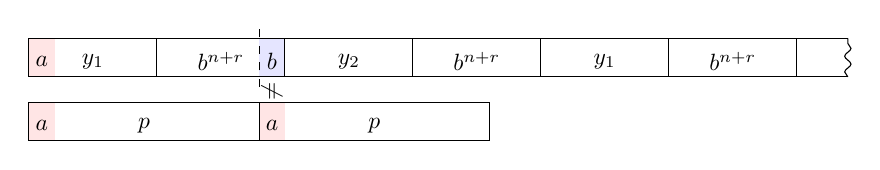
\begin{tikzpicture}[scale=0.65,every node/.style={scale=0.85}]
	\path[fill=red!10] (0,0) rectangle (0.5,0.75);
	\path[fill=red!10] (0,-0.5) rectangle (0.5,-1.25);
	\path[fill=red!10] (4.5,-0.5) rectangle (5,-1.25);
	\path[fill=blue!10] (4.5,0) rectangle (5,0.75);
	
	\draw (0,0) rectangle (15,0.75);
	\draw (0,0) rectangle (15,0.75);
	\draw (15,0) -- (16,0);
	\draw[decorate,decoration={snake,amplitude=.4mm,segment length=2mm}] (16,0) -- (16,0.75);
	\draw (16,0.75) -- (15,0.75);
	
	\draw (2.5,0) -- (2.5,0.75);
	\draw (5,0) -- (5,0.75);
	\draw (7.5,0) -- (7.5,0.75);
	\draw (10,0) -- (10,0.75);
	\draw (12.5,0) -- (12.5,0.75);
	
	\node at (1.25,0.3) {$y_1$};
	\node at (3.75,0.3) {$b^{n+r}$};
	\node at (6.25,0.3) {$y_2$};
	\node at (8.75,0.3) {$b^{n+r}$};
	\node at (11.25,0.3) {$y_1$};
	\node at (13.75,0.3) {$b^{n+r}$};
	
	\draw[dashed] (4.5,-0.2) -- (4.5,0.95);
	
	\node at (4.75,0.3) {$b$};
	\node at (0.25,0.3) {$a$};
	\node at (0.25,-0.95) {$a$};
	\node at (4.75,-0.95) {$a$};
	
	\node[rotate=90] at (4.75,-0.275) {$\neq$};
	
	\draw (0,-0.5) rectangle (4.5,-1.25);
	\draw (4.5,-0.5) rectangle (9,-1.25);
	
	\node at (2.25,-0.95) {$p$};
	\node at (6.75,-0.95) {$p$};
\end{tikzpicture}
			\subcaption{Case $\left\lfloor\frac{|p|}{n+r}\right\rfloor$ is odd\label{fig:repetition:i1}}
		\end{subfigure}
		\begin{subfigure}{\textwidth}
			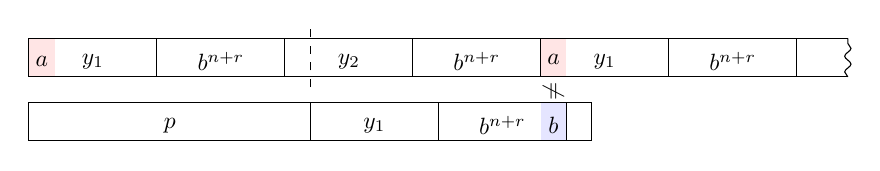
\begin{tikzpicture}[scale=0.65,every node/.style={scale=0.85}]
	\path[fill=red!10] (0,0) rectangle (0.5,0.75);
	\path[fill=blue!10] (10,-0.5) rectangle (10.5,-1.25);
	\path[fill=red!10] (10,0) rectangle (10.5,0.75);
	
	\draw (0,0) rectangle (15,0.75);
	\draw (15,0) -- (16,0);
	\draw[decorate,decoration={snake,amplitude=.4mm,segment length=2mm}] (16,0) -- (16,0.75);
	\draw (16,0.75) -- (15,0.75);
	
	\draw (2.5,0) -- (2.5,0.75);
	\draw (5,0) -- (5,0.75);
	\draw (7.5,0) -- (7.5,0.75);
	\draw (10,0) -- (10,0.75);
	\draw (12.5,0) -- (12.5,0.75);
	
	\node at (1.25,0.3) {$y_1$};
	\node at (3.75,0.3) {$b^{n+r}$};
	\node at (6.25,0.3) {$y_2$};
	\node at (8.75,0.3) {$b^{n+r}$};
	\node at (11.25,0.3) {$y_1$};
	\node at (13.75,0.3) {$b^{n+r}$};
	
	\draw[dashed] (5.5,-0.2) -- (5.5,0.95);
	
	\draw (0,-0.5) rectangle (5.5,-1.25);
	\draw (5.5,-0.5) rectangle (11,-1.25);
	\draw (8,-0.5) -- (8,-1.25);
	\draw (10.5,-0.5) -- (10.5,-1.25);
	
	\node at (2.75,-0.95) {$p$};
	\node at (6.75,-0.95) {$y_1$};
	\node at (9.25,-0.95) {$b^{n+r}$};
	
	\node at (0.25,0.3) {$a$};
	\node at (10.25,0.35) {$a$};
	\node at (10.25,-0.95) {$b$};
	
	\node[rotate=90] at (10.25,-0.275) {$\neq$};
\end{tikzpicture}
			\subcaption{Case $\left\lfloor\frac{|p|}{n+r}\right\rfloor$ is even\label{fig:repetition:i2}}
		\end{subfigure}
		\caption{\label{fig:repetition}}
	\end{figure}
	
	Now, assume $|p|$ is a divisor of $n+r$. Then we can understand the blocks of length $n+r$ as letters of the alphabet $\{b^{n+r},y_1,\dots,y_i\}$. Since there is no $y_i$-block in $v_i$ we have $|p|\geq|v_iy_i|$. Since $p$ starts with $y_1$ and $y_i$ is followed by $b^{n+r}$, $p$ has length at least $|v_ix_i|$.
	
	\emph{Proof of (\ref{prf:short_from_skeleton:i2}).}\ By construction, it is easy to see that $\vec{v}=(v_0,\dots,v_n)$ is a canon-decomposition of $v=v_n$. We prove now by induction on $0\leq i<n$ that $(v_0,\dots,v_{i+1})$ is a complete canon-decomposition of $v_i$. The case $i=0$ is easy to verify since $v_1\in aA^{r-1}b^{2n+r}$. So, let $i\geq1$. Assume there is $u\in\varSigma^*$ with $v_i\presuf u\presuf v_{i+1}$. Let $u$ be of minimal length satisfying this inequality. Then there are two possible cases:
	
	First, suppose $|u|\geq|v_ix_i|$ holds, i.e., the prefix and suffix $u$ overlap in $v_i$ and the overlap contains at most $x_i$ (cf.\ Fig.~\ref{fig:skeleton}). Let $x,y\in\varSigma^*$ such that $u=xx_iv_i=y$. Then we have $|x|=|y|$ and $m:=xx_iy\presuf u$. Hence, by minimality of $u$ we have $|m|\leq|v_i|$ and therefore, by induction hypothesis, $m=v_k$ for some $0< k\leq i$. This implies
	\[v_{k-1}x_{k-1}v_{k-1}=v_k=m=xx_iy\,.\]
	Since $|x|=|y|$ and $|x_i|=|x_{k-1}|$ we have $x_i=x_{k-1}$, which is a contradiction to the construction of the $x_i$'s.
	
	\begin{figure}[H]
		\centering\begin{tikzpicture}[scale=0.65,every node/.style={scale=0.85}]
	\node at (-0.75,0.2){$v_{i+1}=$};
	\node at (-0.75,-0.9){$u=$};
	\node at (-0.75,-1.7){$u=$};
	
	\draw (0,0) rectangle (15,0.75);
	\draw (0, -0.5) rectangle (10,-1.25);
	\draw (5, -1.25) rectangle (15,-2);

	\draw (5,.75) -- (5,0);	
	\draw (6,.75) -- (6,0);
	\draw (9,.75) -- (9,0);
	\draw (10,.75) -- (10,0);
	
	\draw (5,-0.5) -- (5,-2);
	\draw (6,-0.5) -- (6,-2);
	\draw (9,-0.5) -- (9,-2);
	\draw (10,-0.5) -- (10,-2);
	
	\node at (7.5,0.3) {$x_i$};
	\node at (9.5,-0.95) {$y$};
	\node at (5.5,-1.7) {$x$};
	
	\draw[snake=brace] (0,0.8) -- (6,0.8);
	\draw[snake=brace] (9,0.8) -- (15,0.8);
	\draw[snake=brace] (10,-2.05) -- (5,-2.05);
	
	\node at (3,1.1) {$v_i$};
	\node at (12,1.1) {$v_i$};
	\node at (7.5,-2.4) {$m$};
\end{tikzpicture}
		\caption{\label{fig:skeleton}}
	\end{figure}
	
	Now, suppose $|u|<|v_ix_i|$. If $|u|\geq\frac{|v_{i+1}|}{2}$ (i.e., the prefix and suffix $u$ in $v_i$ overlap) then there is a word $m\in\varSigma^*$ such that $m\presuf u$ holds. Hence, by minimality of $u$ and by induction hypothesis we have $m=v_k$ for some $0\leq k\leq i$. Since $|m|<|x_i|=|x_1|$ we have $m=\varepsilon$, i.e., we have $|u|=\frac{|v_{i+1}|}{2}$.
	
	Suppose $|u|\leq\frac{|v_{i+1}|}{2}$ (i.e., the prefix and suffix $u$ in $v_i$ do not overlap). Then there is a word $p\in\varSigma^*$ such that $v_{i+1}=pu$. Since $u$ is a prefix of $v_{i+1}$ and $|p|>\frac{|v_{i+1}|}{2}$, $u$ also is a prefix of $p$. Hence, $p$ is a period of $v_{i+1}$ and we have
	\[|p|=|v_{i+1}|-|u|<|v_{i+1}|-|v_i|=|v_ix_i|\,.\]
	This is a contradiction to property~\ref{prf:short_from_skeleton:i1} stating that $v_ix_i$ is the minimal period of $v_{i+1}$.
	
	So, in both cases we have seen that there is no $v_i\presuf u\presuf v_{i+1}$, i.e., $(v_0,\dots,v_{i+1})$ is a complete canon-decomposition.
	
	Finally, let $0\leq i<n$. Then we have
	\[\calS_r(v)[i]=\pref_r(\inv{v_i}v)=\pref_r(\calS_r(w)[i]\,s)=\calS_r(w)[i]\]
	for some $s\in\varSigma^*$, i.e., $\calS_r(v)=\calS_r(w)$.
\end{proof}

Let $V\in (\varSigma^{\leq r})^*$ be the $r$-skeleton of some word $w\in\varSigma^*$. We call the word $v\in\varSigma^*$ constructed in the proof of Lemma~\ref{lem:short_from_skeleton} the \emph{canonical $r$-instantiation of $V$}.